\section{Results Analysis}

Multidimensional data analysis was performed to determine accurate statistical metrics to optimize the sensor fusion design. A set of signals comrpised of the raw time signals of the compass system, compass filter, full system combined, gyro system, gyro filter, and input heading signal can be observed in Figure \ref{fig:raw_time_signals_full}. In order to quantify the error of each sensor system output, the difference $\delta_k$ was determined for each signal $y_k$ with the input heading signal $y_i$. A set of new sensor data was created compounding by these differences $\delta_n$. To adequately quantify the error of each sensor output, analysis must be performed throughout a range of cutoff frequencies since this could drastically change the response of the full system. It is not expected that the independent system outputs for the gyro and compass systems would change over a range of cutoff frequencies since they are decoupled from this variation. However, the filter's response and full system response would change since they depend on the cutoff frequencies. Before describing the data analysis performed, the time responses of the signal's response to the heading input is observed in Figures \ref{fig:raw_time_signals_full} to \ref{fig:raw_error_signals_transient} for a 350 second simulation.

\begin{figure}[H]
    \centering
    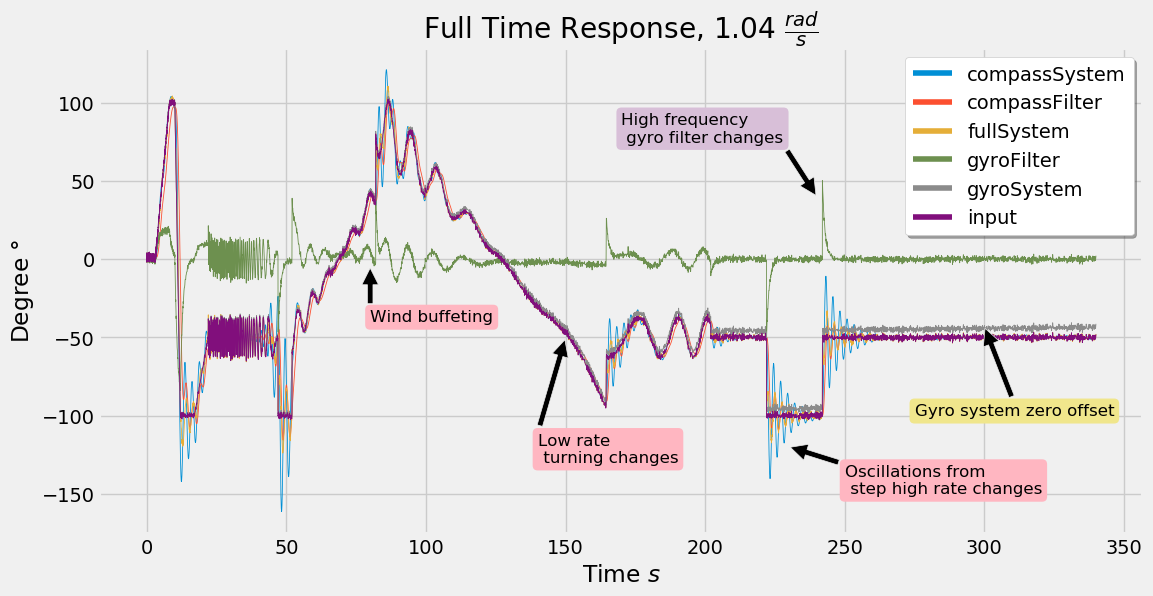
\includegraphics[width=\linewidth]{img/allSignalsFullTimeResponse_1_0476.png}
    \caption{All signals response to the heading input signal.}
    \label{fig:raw_time_signals_full}
\end{figure}

From Figure \ref{fig:raw_time_errors_full} it can be noticed that the full system error is considerably smaller than the error of each individual sensor due to the complementary filters. It can even be noticed that at very high frequencies such as near second 50, even the gyro filter begins oscillating potentially due to magnitude attenuation described in Figure \ref{fig:gyro_bode}.

The gyro filter output error mostly trails the inverse of the full system response in Figure \ref{fig:raw_time_errors_full}. At most points within the heading flight, the gyro filter output value in Figure \ref{fig:raw_time_signals_full} is near zero. Its magnitude suddenly increases to respond to higher frequency changes such as observed by the 40s chirp sine, 100s wind buffeting, 175s turning rates, or 225s step changes. This is expected due to the complementary filter mechanism that transfers all higher frequency excitation above the modelled 1.04 $\frac{rad}{s}$ cutoff frequency.

\begin{figure}[H]
    \centering
    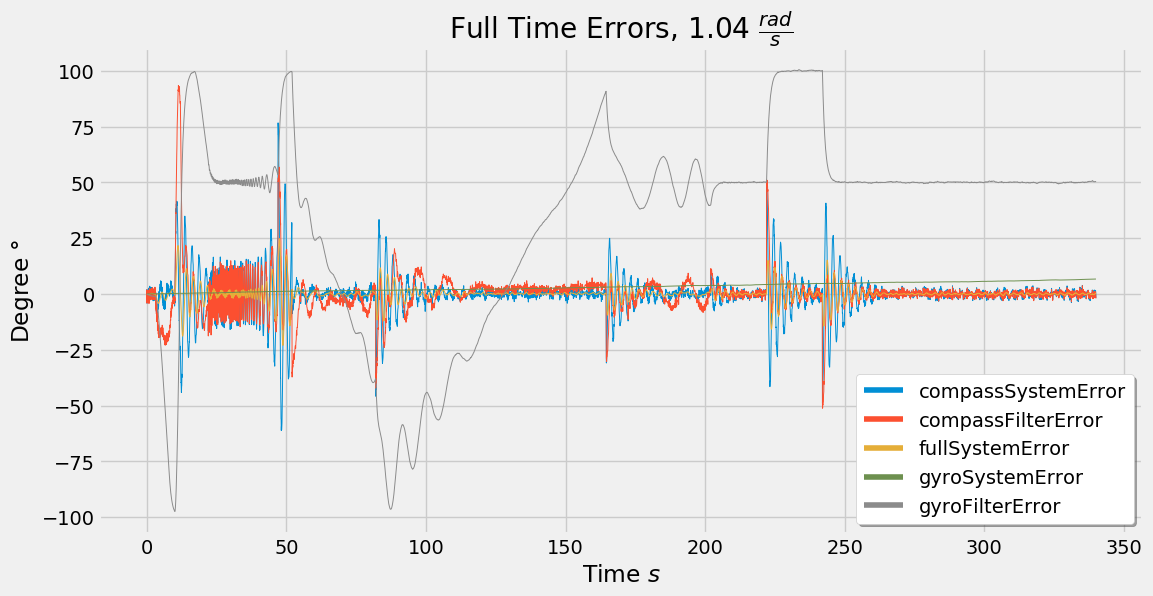
\includegraphics[width=\linewidth]{img/errorSignalsFullTimeResponse_1_0476.png}
    \caption{Error difference of each system signal for the full input heading signal.}
    \label{fig:raw_time_errors_full}
\end{figure}

The gyro system's zero offset from mechanical flight imperfections can be observed around 300 s, although for longer simulations that were run, it continuously increased which meant that high frequency oscillations were not accurately captured.

The compass filter and compass system trail the full system response at low frequencies, and these sensors oscillate at high frequency changes as observed in time 10s in Figure \ref{fig:raw_time_signals_transient}. Note that the full system oscillations are much lower since the complementary filter design compensates at high frequencies and reduces the compass system input into the response.

\begin{figure}[H]
\centering
\begin{subfigure}{0.495\textwidth}
  \centering
  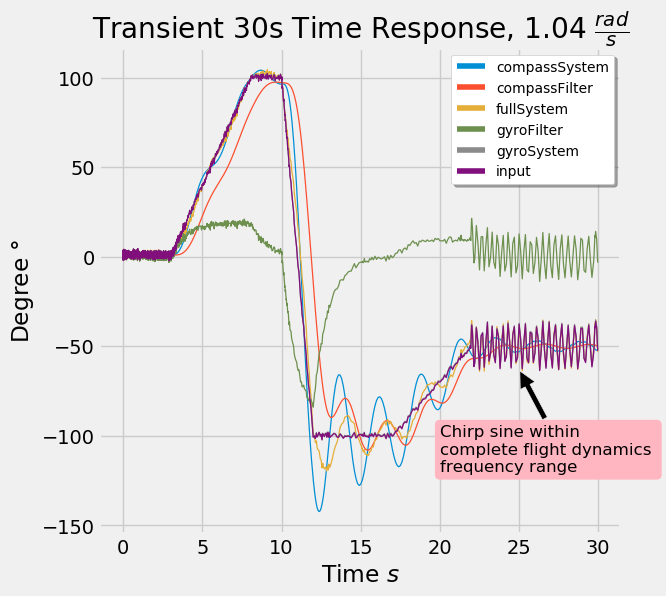
\includegraphics[width=\linewidth]{img/allSignalsTimeResponse30s_1_0476.png}
  \caption{Initial 30s response of all system signals. Note that the \texttt{input} legend refers to the heading signal.}
  \label{fig:raw_time_signals_transient}
\end{subfigure}
\begin{subfigure}{0.495\textwidth}
  \centering
  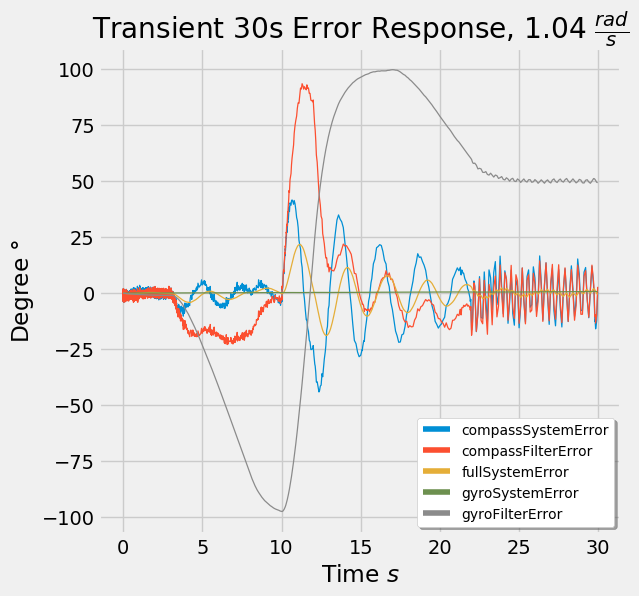
\includegraphics[width=\linewidth]{img/errorSignalsTimeResponse30s_1_0476.png}
  \caption{Error with the heading input of all the system signals. Note that the \texttt{input} legend refers to the heading signal.}
  \label{fig:raw_error_signals_transient}
\end{subfigure}
\caption{All signals initial 30s response.}
\end{figure}



